\section*{Decision 3: Querying Tycoons to Get Available Routes}

\subsection*{Status}
Accepted

\subsection*{Architectural Summary}
In the context of enhancing the TrIP system's ability to provide optimized travel options, we face the challenge of efficiently querying multiple tycoon systems to gather route information that aligns with passenger preferences and existing subscriptions.

\subsection*{Concern}
The concern is to facilitate a seamless travel planning experience for passengers by ensuring the system can accurately and efficiently gather available route options from various tycoon systems and present them based on the user's criteria of price, time, and subscription status.

\subsection*{Context}
The decision is centered on the system's interface with tycoon systems to retrieve and optimize route data, which impacts the functionality and performance of the terminal's route planning features for the passengers.

\subsection*{Criteria}
The key criteria for the decision include:
\begin{itemize}
    \item User-friendly passenger interface.
    \item Comprehensive and diverse route options.
    \item Accurate representation of options based on multiple factors.
    \item Streamlined integration with multiple tycoon systems.
\end{itemize}

\subsection*{Option 1: Direct Tycoon Integration}
Terminals directly interface with each tycoon system and the central database to collate route options. The route optimizer processes this data to present optimal travel solutions.
\begin{figure}[ht]
    \centering
    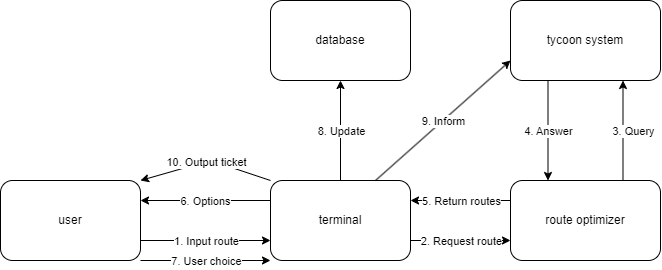
\includegraphics[width=0.5\textwidth]{drawings/decision3_drawings/direct.png}
    \caption{Direct Data Management Interface}
    \label{fig:direct-data-interface}
\end{figure}

\subsection*{Option 2: Centralized Data Management Interface}
A central data management module acts as an intermediary between terminals and tycoon systems, standardizing and aggregating data before it is processed by the route optimizer.
\begin{figure}[ht]
    \centering
    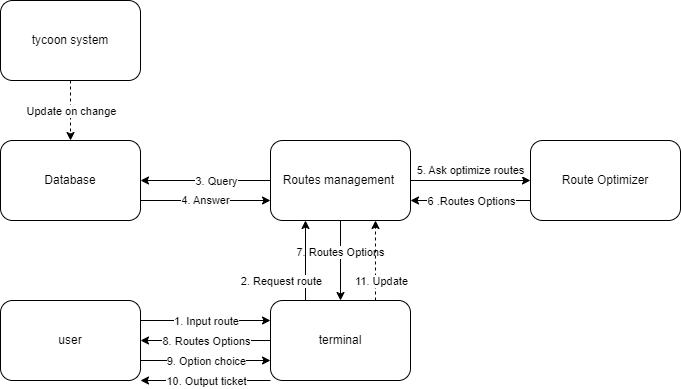
\includegraphics[width=0.5\textwidth]{drawings/decision3_drawings/centralized.png}
    \caption{Centralized Data Management Interface}
    \label{fig:centralized-data-interface}
\end{figure}
  
\subsection*{Decision}
We have decided to proceed with Option 2: Centralized Data Management Interface. This decision is based on the module's ability to simplify the data flow between systems and to effectively manage the complexity of integrating with multiple tycoon systems. The introduction of a separate data management module will allow for greater flexibility and scalability.

\subsection*{Consequences}
\textbf{Positive Consequences:}
\begin{itemize}
    \item Simplified data flow between the trip system and tycoons.
    \item Improved scalability and maintainability of the system.
    \item Easier to integrate with current and future tycoon systems.
\end{itemize}
\textbf{Negative Consequences:}
\begin{itemize}
    \item Initial development and integration effort for the new module.
    \item Potential complexity in data synchronization between modules.
\end{itemize}
This approach is expected to provide a solid foundation for the system's scalability and adaptability to evolving requirements and stakeholder needs.